\section{Exercise 5 - Inverse Gray Code's and Benchmarks}
Presented below the results of the benchmark on the Student's machine. The specs of the machine are shown in the listing below the figure with the results.

\begin{figure}[h]
    \begin{center}
        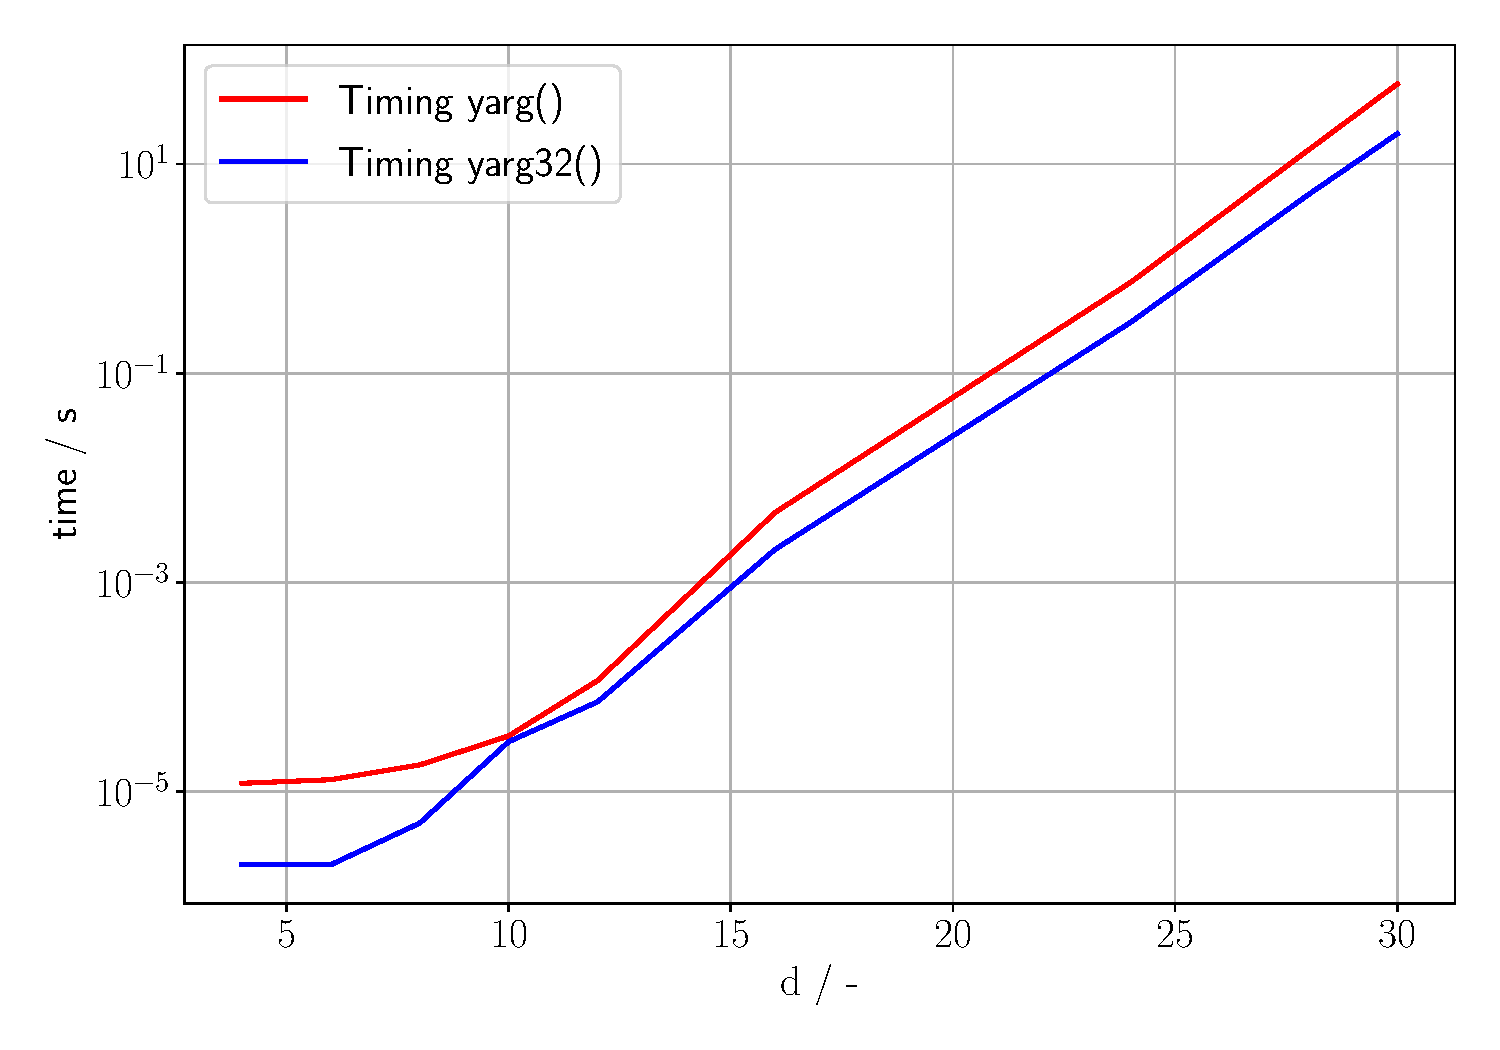
\includegraphics[width= 0.88\linewidth]{figures/task_5_plot.pdf} 
        \label{ref_plot_task_5}
        \caption{Benchmark both algorithms - \texttt{yarg32()} is faster than \texttt{yarg()} for all feasible values of $d$}
    \end{center}
\end{figure}


\begin{lstlisting}[language=bash, title=Linux Terminal Output of \texttt{lscpu}]
    tellocam@DESKTOP-0AFJNHI:~/Projects/HPC/Exercise_1/Quell_Kodierung/CLANG$ lscpu
    Architecture:                    x86_64
    CPU op-mode(s):                  32-bit, 64-bit
    Byte Order:                      Little Endian
    Address sizes:                   39 bits physical, 48 bits virtual
    CPU(s):                          12
    On-line CPU(s) list:             0-11
    Thread(s) per core:              2
    Core(s) per socket:              6
    Socket(s):                       1
    Vendor ID:                       GenuineIntel
    CPU family:                      6
    Model:                           158
    Model name:                      Intel(R) Core(TM) i7-8700K CPU @ 3.70GHz
    Stepping:                        10
    CPU MHz:                         3696.001
    BogoMIPS:                        7392.00
    Hypervisor vendor:               Microsoft
    Virtualization type:             full
    L1d cache:                       192 KiB
    L1i cache:                       192 KiB
    L2 cache:                        1.5 MiB
    L3 cache:                        12 MiB
 
\end{lstlisting}

\pagebreak

In the listing below, both the algorithms as well as the experimental setup is shown. In line 13 - 20 for example, the \texttt{clock()} function is used which counts the
number of clock ticks during the execution time. If one divides that by \texttt{CLOCKS\_PER\_SEC} which is constant, one obtains an acceptable execution timing of all yargcode calculations for
the hypercube.

\begin{lstlisting}[language=C, title=C Language Listing for EX1.5]
    typedef unsigned int uint;
    uint gray(uint num){
        // Same as in Exercise 1.4
    }
    uint yarg(uint num){
        // Same as in Exercise 1.4
    }
 
    uint yarg32(uint num){
        // Same as in Exercise 1.4
    }

    int main()
    {
        int d = 30;
        clock_t start = clock();
        for (int j = 1; j < pow(2, d); j++)
        {
            yarg(j);
        }
        clock_t res = clock() - start;
        printf("yarg(): %f s\n", (double)res / CLOCKS_PER_SEC);
    
        start = clock();
        for (int j = 1; j < pow(2, d); j++)
        {
            yarg32(j);
        }
        res = clock() - start;
        printf("yarg32(): %f s\n", (double)res / CLOCKS_PER_SEC);
    
        return 0;
    }
\end{lstlisting}

\pagebreak



\section{Exercise 6 - not done..}

\section{Exercise 7 - not done..}